\documentclass[conference]{IEEEtran}
\usepackage[utf8]{inputenc}
\usepackage[T1]{fontenc}
\usepackage[spanish,es-tabla]{babel}
\usepackage{booktabs}
\usepackage{graphicx}
\usepackage{url}
\begin{document}
\title{Detección binaria de daño visible en edificaciones mediante imágenes satelitales PRE/POST: estudio comparativo en México y Palu}
\author{\IEEEauthorblockN{Grupo 04}
\IEEEauthorblockA{Aplicaciones de IA en Estructuras}}
\maketitle
\begin{abstract}
Se implementó un sistema para clasificar edificaciones como dañadas o no dañadas mediante pares de imágenes satelitales PRE/POST del conjunto xBD. Se integraron 106\,540 edificios válidos de un terremoto en México y un tsunami en Palu, con 8\,660 edificios anotados con daño. Se respetaron las particiones de origen por escena. En la validación conjunta (19\,537 edificios), Random Forest obtuvo F1 de 0.5703 y AP de 0.5999; DINOv2 con XGBoost, F1 de 0.6897 y AP de 0.7400; ProtoNet DINO, F1 de 0.6784 y AP de 0.7195; y Hybrid, F1 de 0.7341 y AP de 0.7768. Se presentan resultados de validación, sin evaluación final reservada de prueba. El predominio de casos positivos en Palu limita la extrapolación del rendimiento global entre eventos.
\end{abstract}
\begin{IEEEkeywords}
clasificación binaria, daño visible, imágenes satelitales, xBD, DINOv2, postdesastre
\end{IEEEkeywords}
\section{Introducción}
La identificación preliminar de edificaciones afectadas puede apoyar la priorización de inspecciones después de un terremoto o un tsunami. La comparación de imágenes anteriores y posteriores a un evento permite reconocer cambios visibles, pero no constituye por sí misma una verificación estructural. Este trabajo compara diferentes modelos de clasificación binaria a nivel de edificio usando datos de dos eventos de xBD \cite{xbd}.
\section{Datos y metodología}
\subsection{Fuente y clasificación}
Se utilizaron 385 escenas con anotaciones válidas de México y Palu: 106\,540 edificios, de los cuales 8\,660 presentan daño. La variable binaria asigna 0 a \texttt{no-damage} y 1 a \texttt{minor-damage}, \texttt{major-damage} y \texttt{destroyed}. Se excluyeron 722 registros \texttt{un-classified}.
\begin{table}[t]
\centering
\caption{Distribución del conjunto multievento}
\label{tab:datos}
\begin{tabular}{lrrr}
\toprule
Evento & Edificios & Dañados & Sin daño \\
\midrule
México & 51\,362 & 278 & 51\,084 \\
Palu & 55\,178 & 8\,382 & 46\,796 \\
\midrule
Total & 106\,540 & 8\,660 & 97\,880 \\
\bottomrule
\end{tabular}
\end{table}
\subsection{Preparación y particiones}
Se procesaron TIFF y anotaciones JSON, se verificaron pares PRE/POST y se generaron recortes por polígono de edificio. Las imágenes RGB (1024 $\times$ 1024 píxeles) contenían valores \texttt{int16} en el rango 0--255. Se comprobó el rango y se convirtió exactamente a \texttt{uint8}, sin modificar la intensidad original. Para cada edificio se empleó la misma ventana en PRE y POST con 12 píxeles de contexto, salida de 224 $\times$ 224 y redimensionamiento bilineal. Cuando la ventana sobrepasa el borde se reflejan los píxeles periféricos para evitar franjas negras artificiales, sin reconstruir detalles ausentes. Este tratamiento no corrige automáticamente el registro geométrico. Se mantienen particiones de origen: \texttt{tier1} para entrenamiento (63\,189 edificios), \texttt{hold} para validación (19\,537) y \texttt{test} para evaluación reservada (23\,814), sin mezclar escenas entre conjuntos.
\subsection{Arquitecturas}
Se desarrollaron Random Forest, DINOv2 + XGBoost y ProtoNet DINO, además de un ensamble Hybrid obtenido mediante promedio de probabilidades de modelos con predicciones compatibles. ProtoNet DINO emplea representaciones visuales y prototipos de clase; se evaluó con el mismo conjunto de validación. Hybrid no constituye un entrenamiento independiente. Se inició ResNet18 Early Fusion con 20 épocas máximas y lotes de 8, pero su ejecución no se completó al cierre del estudio.
\subsection{Registro del apoyo de inteligencia artificial}
Se utilizó ChatGPT (OpenAI) como apoyo para revisar alternativas de procesamiento, interpretar errores del programa y métricas de validación, y organizar documentación técnica. Se registraron 29 consultas técnicas representativas en la bitácora \texttt{TF3/docs/BITACORA\_USO\_IA.md}, con consultas reformuladas, asistencia obtenida y comprobaciones disponibles; es una selección temática y no una transcripción literal ni exhaustiva. Las decisiones de clasificación, la ejecución de los entrenamientos y la revisión de sus resultados correspondieron al equipo. Las métricas se extrajeron de los registros de CIMLAB AI y no fueron estimadas mediante el modelo conversacional. El apoyo de IA no sustituye el análisis independiente ni la evaluación reservada.

\section{Protocolo de evaluación}
La selección se realiza en validación y se informa precisión promedio (AP), F1, recall y precisión respecto a daño visible. La partición de prueba no se utiliza para elegir los modelos ni sus umbrales.
\section{Resultados y discusión}
\begin{table}[t]
\centering
\caption{Resultados registrados en validación conjunta}
\label{tab:metricas}
\begin{tabular}{lrrrr}
\toprule
Modelo & AP & F1 & Rec. & Prec. \\
\midrule
Random Forest & 0.5999 & 0.5703 & 0.5169 & 0.6360 \\
DINOv2 + XGBoost & 0.7400 & 0.6897 & 0.6033 & 0.8050 \\
ProtoNet DINO & 0.7195 & 0.6784 & 0.6386 & 0.7235 \\
Hybrid & \textbf{0.7768} & \textbf{0.7341} & \textbf{0.6796} & 0.7980 \\
\bottomrule
\end{tabular}
\end{table}

\begin{table}[t]
\centering
\caption{Conteos de confusión en validación (19\,537 edificios)}
\label{tab:confusion}
\begin{tabular}{lrrrr}
\toprule
Modelo & TP & FP & FN & TN \\
\midrule
Random Forest & 718 & 411 & 671 & 17\,737 \\
DINOv2 + XGBoost & 838 & 203 & 551 & 17\,945 \\
ProtoNet DINO & 887 & 339 & 502 & 17\,809 \\
Hybrid & 944 & 239 & 445 & 17\,909 \\
\bottomrule
\end{tabular}
\end{table}
\begin{figure}[t]
\centering
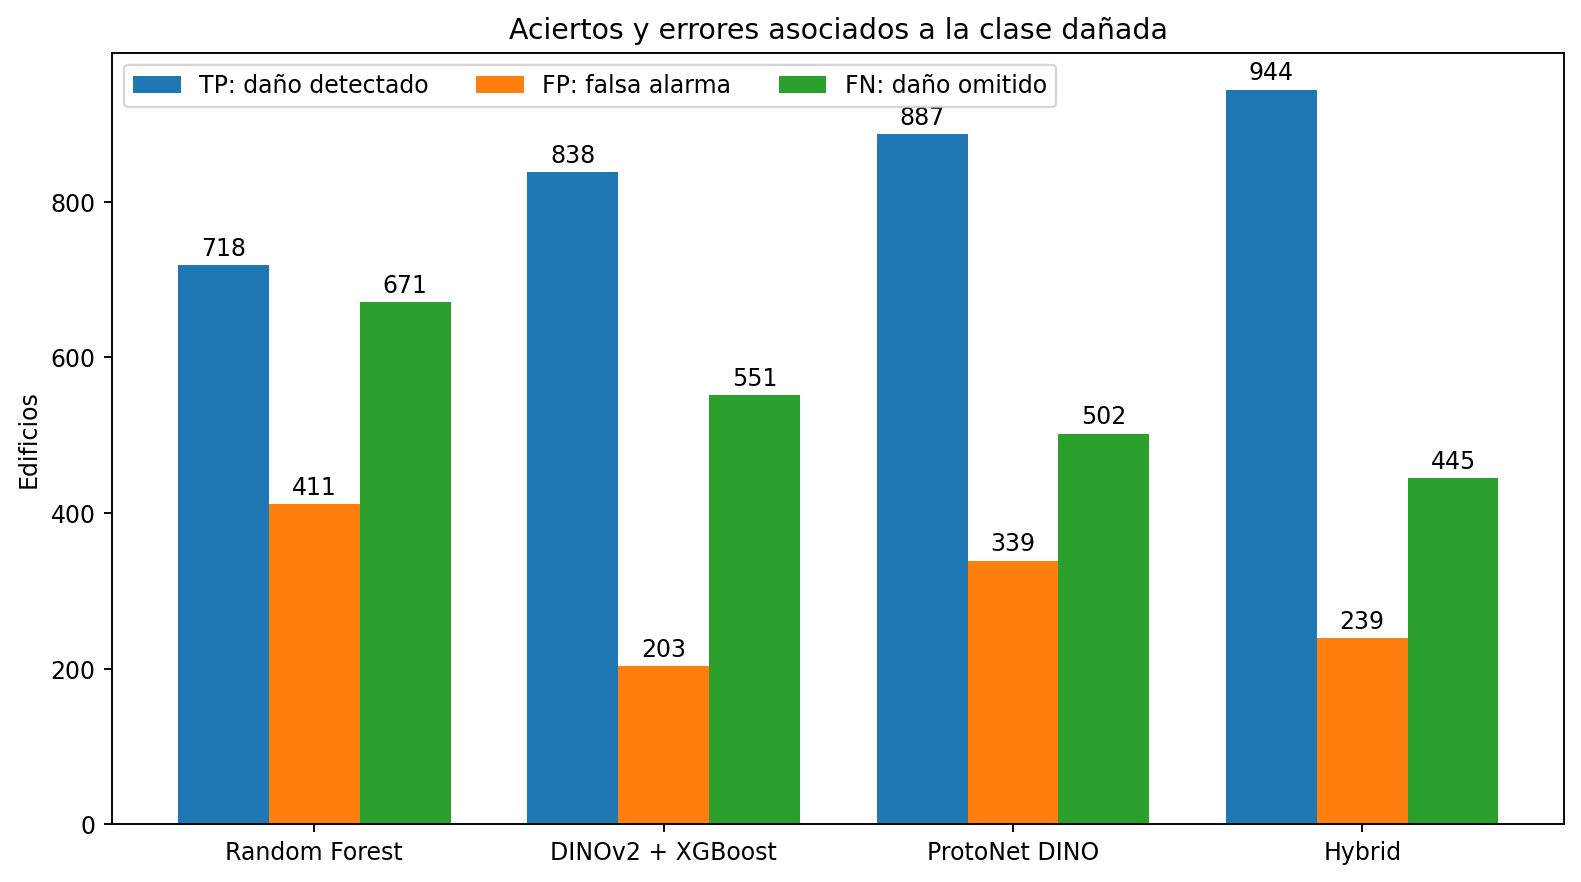
\includegraphics[width=\columnwidth]{../resultados/figuras/comparacion_fp_fn_tp.png}
\caption{Verdaderos positivos (TP), falsos positivos (FP) y falsos negativos (FN) en validación.}
\label{fig:errores}
\end{figure}

Para ProtoNet DINO, los conteos de la tabla provienen del registro del modelo. Los otros se reconstruyeron mediante precisión y recall reportados con cuatro decimales, conocidos 1\,389 positivos y 18\,148 negativos; las cifras recuperadas reproducen asimismo el F1 reportado. Las matrices de confusión individuales se publican como figuras en el repositorio. Hybrid obtuvo 445 FN y 239 FP, mientras DINOv2 + XGBoost obtuvo 551 FN y 203 FP: el ensamble recupera más casos de daño a costa de algunas falsas alarmas adicionales. No se dispone de archivos de predicción por edificio que permitan auditar errores individuales.

Entre los resultados cuantitativos verificados, el ensamble presenta el mayor F1 y AP. En relación con DINOv2 + XGBoost, incrementa el F1 en 0.0444 y el recall en 0.0763, con una disminución de precisión de 0.0070. Esta ventaja debe interpretarse con cautela: 8\,382 de los 8\,660 edificios dañados corresponden a Palu (96.8\,\%), por lo que el desempeño agregado puede no representar el rendimiento en México.

ProtoNet DINO registró F1 de 0.6784 y AP de 0.7195. La última comparación del ensamble Hybrid registró F1 de 0.7341 y AP de 0.7768. Su composición exacta no consta en los archivos suministrados. Como observación de un experimento no finalizado, ResNet18 Early Fusion registró AP de 0.8135 y F1 de 0.7709 en la primera época; en la segunda, AP de 0.7432 y F1 de 0.6662. No se incluyen estos valores en la tabla comparativa por no disponer de un entrenamiento concluido. Tampoco se reporta evaluación final con \texttt{test} ni métricas separadas por evento.
\section{Conclusiones}
Los datos de México y Palu se integraron en un conjunto binario de 106\,540 edificios con particiones por escena. En validación conjunta, DINOv2 + XGBoost superó a Random Forest y el ensamble Hybrid alcanzó F1 de 0.7341 y AP de 0.7768. La elevada concentración de edificios dañados en Palu limita la transferencia de estas cifras a otros eventos. La clasificación se restringe al daño visible desde satélite y no sustituye la inspección estructural en campo. La evaluación reservada y el análisis desagregado por evento quedan como trabajo posterior.
\begin{thebibliography}{4}
\bibitem{xbd} R. Gupta \emph{et al.}, ``xBD: A Dataset for Assessing Building Damage from Satellite Imagery,'' 2019. [En línea]. Disponible: \url{https://arxiv.org/abs/1911.09296}
\bibitem{xview} xView2, ``Dataset and challenge.'' [En línea]. Disponible: \url{https://www.xview2.org/}
\bibitem{baseline} DIU, ``xView2 Baseline.'' [En línea]. Disponible: \url{https://github.com/DIUx-xView/xView2_baseline}
\bibitem{vds} B. Yu y R. Barter, \emph{Veridical Data Science}. MIT Press, 2024.
\end{thebibliography}
\end{document}
